%!TEX root = ../NCVC6.tex

\mysection{読み込み条件を変えてGコードの生成}

\vspace*{1zh}
 1つ目の小細工ポイントです。
図\ref{fig:setup} のように切削レイヤも原点レイヤもG54に関する情報のみを読み込むように設定し[再読み込み]ボタンを押すと、
図\ref{fig:g54} のようにデータを絞ることができます。

%\begin{figure}[H]
%\centering
%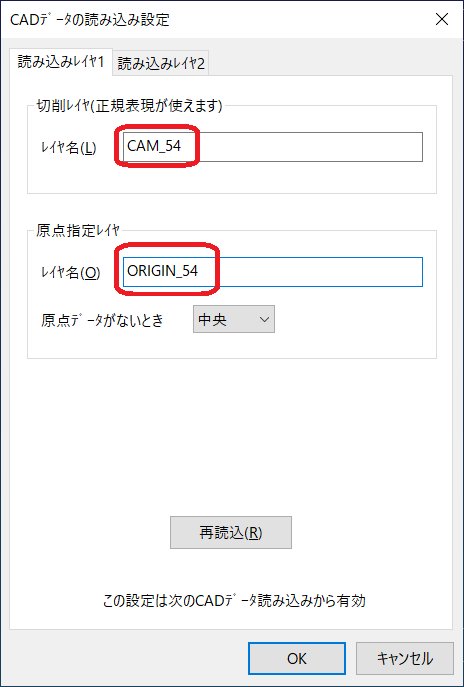
\includegraphics[scale=0.7]{No3/fig/setup.png}
%\caption{CADデータの読み込み設定}
%\label{fig:setup}
%\end{figure}

%\begin{figure}[H]
%\centering
%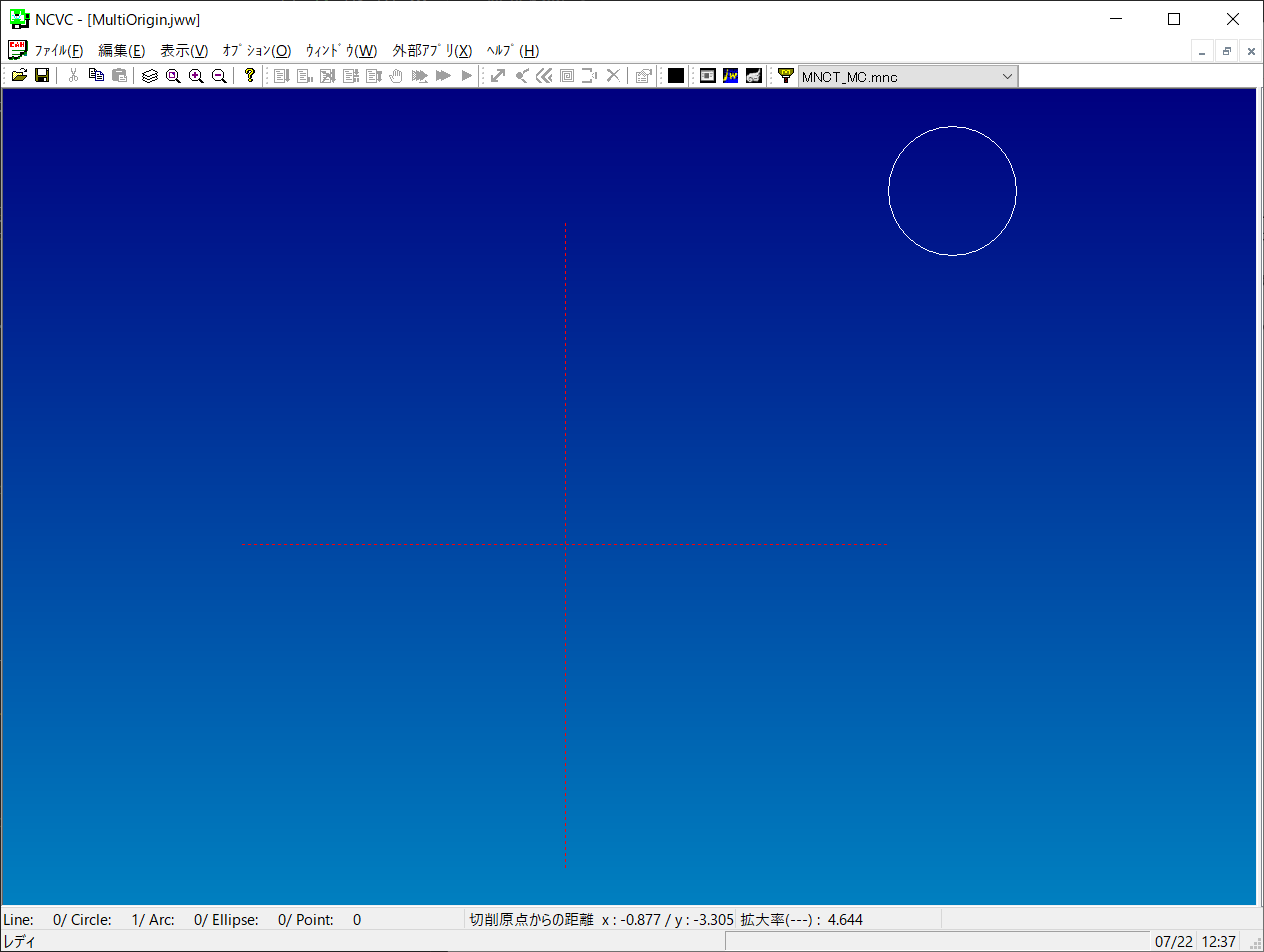
\includegraphics[scale=0.5]{No3/fig/g54.png}
%\caption{G54に関するデータだけを読み込み}
%\label{fig:g54}
%\end{figure}

 この状態で普通にGコードを生成してください。
あとで手作業による修正があるので、カスタムヘッダーはそのままで結構です。
これをワーク座標系分繰り返します(このサンプルではG54からG57までの4回)。

 ただし、それぞれのデータがわかるよう図\ref{fig:makedlg} のように出力ファイル名を変えてください。
上書きしてしまうとやり直しです。

%\begin{figure}[H]
%\centering
%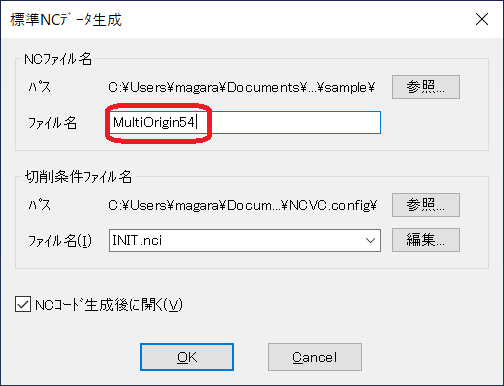
\includegraphics[scale=0.7]{No3/fig/makedlg.png}
%\caption{Gコードの出力}
%\label{fig:makedlg}
%\end{figure}
